\section{在 Linux 系统上安装 CUDA 工具包}

本章讲解如何在 Linux 系统上安装 CUDA 工具包。假设你正在使用前文介绍过的 WSL 工具，首先打开"开始"菜单，搜索"命令
提示符"并点击打开，然后输入 \texttt{wsl} 即可在当前 Windows 系统上启动 Linux 子系统。

\subsection{检查nvcc}

现在检查 \texttt{nvcc} 编译器是否已安装在 Ubuntu 系统中。启动 Ubuntu 后，终端提示 \texttt{command not found}，
说明 \texttt{nvcc} 尚未安装。

\begin{figure}
    \centering
    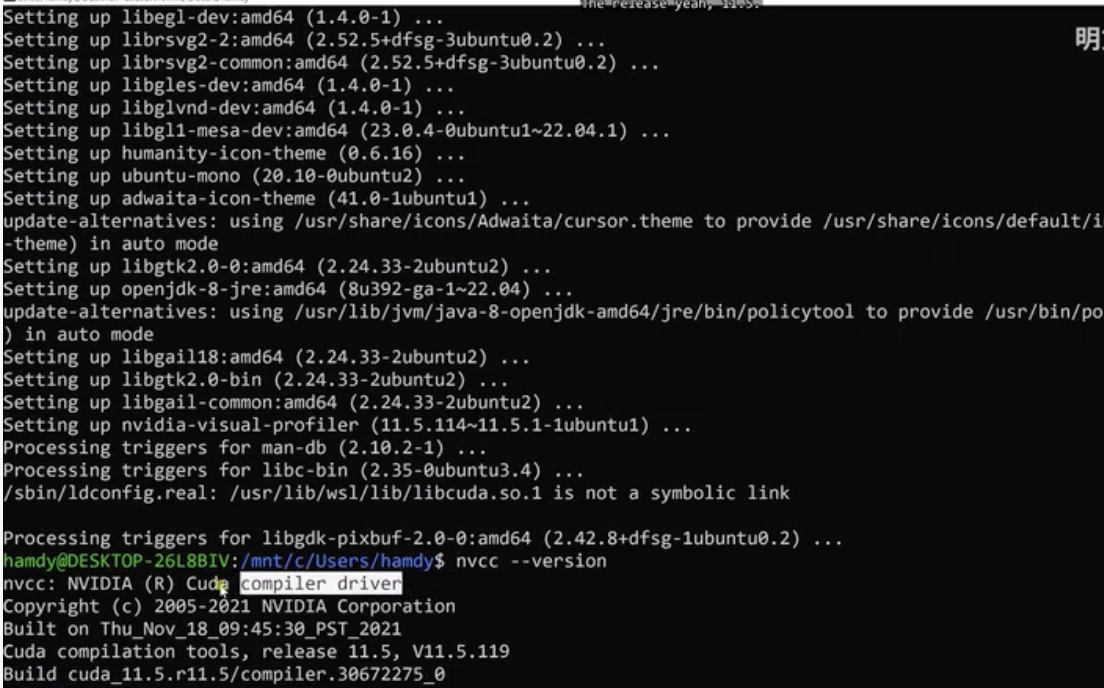
\includegraphics[width=0.75\linewidth]{resources/cuda-060.png}
    \caption{}
    \label{fig:placeholder}
\end{figure}

\subsection{安装CUDA工具包}

需要安装 CUDA 工具包才能使用 \texttt{nvcc} 编译器。打开 CUDA 工具包下载页面，选择操作系统、架构以及发行版本。
有多种发行版可选，这里选择 Ubuntu；如果你使用的是 WSL，也可以选择 WSL-Ubuntu。接着会看到三个安装选项：其中两个
先下载本地安装包（标为 Local），中间那个则是通过网络直接安装（Network）。不过，最简单、最不容易出错的方式是直接使
用 \texttt{apt} 安装。

再检查一次 \texttt{nvcc} 版本，虽然提示命令未找到，但第二行给出了安装建议：
\begin{verbatim}
sudo apt install nvidia-cuda-toolkit
\end{verbatim}

复制这条指令并在终端中输入，然后输入密码。系统会询问是否继续，输入 Y 确认即可。安装过程大约需要 30-40 分钟，请耐心等
待。CUDA 工具包安装完成后，你将拥有 \texttt{nvcc} 编译器以及前文介绍的所有其他功能。再次检查 \texttt{nvcc} 编译器版
本，可以看到 CUDA 编译器已成功安装（版本 11.5），输出第一行显示 \texttt{nvcc: NVIDIA (R) Cuda compiler driver}，
表示 CUDA 工具包已就绪，对入门来说已经足够了。

另外提醒一点：如果你按照官网的步骤操作，可能会遇到一些依赖问题或错误。因此建议一开始先使用上述 \texttt{apt} 指令，它简
单且不易出错。等你熟悉之后，需要更新 CUDA 工具包时，再到 CUDA 官网选择适合你系统的最新版本进行安装。
